\documentclass[12pt]{handout}
%\usepackage{add-copyright}

\title{Homework 1}
\course{Math 1181H}
\date{Due Tuesday, August 28, 2012}
\author{Jim Fowler}

\usepackage[T1]{fontenc}
\usepackage{lmodern}
\usepackage{hyperref}

\newcommand{\peem}{\textsc{p.m.}}
\newcommand{\ayem}{\textsc{a.m.}}

\usepackage{nopageno}
\usepackage{multicol}
\geometry{margin=1cm}
%\geometry{landscape,margin=0.25in,bottom=0.25in,left=0.5in,right=0.5in}
\usepackage{tabularx}
\usepackage{rotating}

\setlength{\parindent}{0in}
\setlength{\parskip}{0in}
\usepackage{calc}

\begin{document}
\maketitle

Welcome to Math~1181H.  Yes, this is \textit{math}---but what's math?
If we look up $\mu\alpha\theta$ in a Greek-English lexicon:
\begin{center}
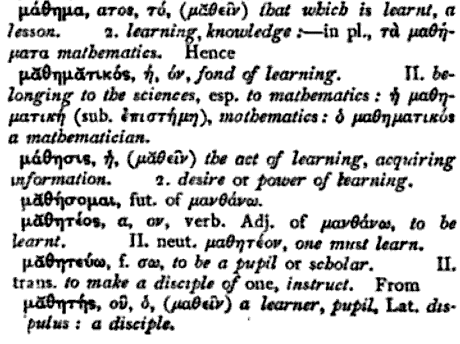
\includegraphics[width=3.5in]{math-definition.png}
\end{center}
Indeed, mathematics epitomizes learning, but this learning comes at the price of discipline.  This is the first of 16 homework assignments to provide this discipline.







\subsection*{Show your work}
When you ``solve'' a problem, the goal is not merely to give a correct answer!  Each problem has a story, and you should \textit{tell the story} by clearly explaining your argument.


\subsection*{The four boxed problems will be graded}
Even if you don't do all the assigned problems (though you should!), the four boxed problems will be graded.

\section*{Assigned Problems}

From \textsection 1.5 (starting on page 22),
do problems 5, \fbox{6}, 7, 17, 27, 35.
\vspace{1ex}

From \textsection 1.6 (starting on page 30),
do problems \fbox{2}, 3, 5, 7.
\vspace{1ex}

From \textsection 1.7 (starting on page 37),
do problems 3, 5, \fbox{6}, 7, 9, 11, 19, 21.
\vspace{1ex}

From \textsection 2.3 (starting on page 58),
do problems 5, 17, \fbox{18}, 21, 23, 39.
\vspace{1ex}


\end{document}
